\documentclass[conference]{IEEEtran}
\IEEEoverridecommandlockouts
\usepackage{fontspec}
\setmainfont{texgyretermes-regular.otf}[BoldFont=texgyretermes-bold.otf,ItalicFont=texgyretermes-italic.otf,BoldItalicFont=texgyretermes-bolditalic.otf]
\setsansfont{texgyreheros-regular.otf}[BoldFont=texgyreheros-bold.otf,ItalicFont=texgyreheros-italic.otf,BoldItalicFont=texgyreheros-bolditalic.otf]
\setmonofont{texgyrecursor-regular.otf}[BoldFont=texgyrecursor-bold.otf,ItalicFont=texgyrecursor-italic.otf,BoldItalicFont=texgyrecursor-bolditalic.otf,Scale=MatchLowercase]
\usepackage{cite}
\usepackage{amsmath,amssymb,amsfonts}
\usepackage{graphicx}
\usepackage{textcomp}
\usepackage{xcolor}
\usepackage{booktabs}
\usepackage{array}
\usepackage{tabularx}
\usepackage{balance}
\usepackage{url}
\usepackage[hidelinks]{hyperref}
\def\BibTeX{{\rm B\kern-.05em{\sc i\kern-.025em b}\kern-.08em
    T\kern-.1667em\lower.7ex\hbox{E}\kern-.125em X}}
\setlength{\textfloatsep}{8pt plus 2pt minus 2pt}
\setlength{\floatsep}{7pt plus 2pt minus 2pt}
\setlength{\intextsep}{7pt plus 2pt minus 2pt}
\setlength{\abovecaptionskip}{3pt}
\renewcommand{\topfraction}{0.95}
\renewcommand{\bottomfraction}{0.95}
\renewcommand{\textfraction}{0.05}
\renewcommand{\floatpagefraction}{0.85}

\begin{document}

\title{ReviewIQ: A Unified NLP, Deep Learning and Advanced Machine Learning Framework for Review Sentiment Classification, Aspect Intelligence and Grounded Question Answering}

\author{\IEEEauthorblockN{Nidhi Bhawari, Aarti Sakpal, Gayatri Patil and Prachi Wakode}
\IEEEauthorblockA{\textit{Vidyalankar Institute of Technology}\\
Mumbai, India}
\and
\IEEEauthorblockN{Prof. Sneha Annappanavar}
\IEEEauthorblockA{\textit{Project Guide}\\
\textit{Vidyalankar Institute of Technology}\\
Mumbai, India}}

\maketitle

\begin{abstract}
Online product reviews are abundant but unstructured, and most published systems address a single task in isolation. This paper presents ReviewIQ, an end-to-end framework that combines classical natural language processing (NLP), deep learning (DL) and advanced machine learning (AML) to turn raw Amazon Electronics reviews into decisions for two audiences: buyers and sellers. On a 50{,}000-review sample we (i) classify review sentiment into positive, neutral and negative with five models on a single shared test split, including a bidirectional LSTM with attention trained from scratch and a fine-tuned DistilBERT; (ii) derive aspect-level sentiment, topics and clusters; (iii) predict review helpfulness with tuned XGBoost; (iv) flag potentially suspicious reviews with an unsupervised Isolation Forest; and (v) answer product-scoped questions through semantic retrieval with a similarity-floor guardrail. The BiLSTM reaches 88.8\% accuracy and the highest macro-F1 (0.718), significantly above a TF-IDF SVM (+0.025, 95\% bootstrap CI [0.010, 0.039]), while DistilBERT achieves the highest accuracy (89.9\%) despite seeing only 6{,}000 training reviews; the macro-F1 difference between the two neural models is not statistically significant. Battery is the most criticised aspect (20.2\% negative mentions). The guardrail rejects 95.6\% of plausible-but-unanswerable and 100\% of off-topic questions while accepting 97.8\% of answerable ones. A three-seed ablation shows that class weighting, not attention, drives most of the LSTM's macro-F1 gain, and that an unweighted LSTM matches DistilBERT's accuracy. Label noise, sampling bias and other limitations are discussed explicitly.
\end{abstract}

\begin{IEEEkeywords}
sentiment analysis, LSTM, attention, DistilBERT, aspect-based sentiment analysis, XGBoost, Isolation Forest, retrieval-augmented generation, product reviews
\end{IEEEkeywords}

\section{Introduction}
Customer reviews influence purchasing decisions and guide product development, yet a single popular product can attract thousands of free-text opinions that no person can read in full. Automated analysis is therefore central to modern e-commerce. The literature, however, tends to treat the associated problems separately: sentiment classification \cite{pang2002thumbs,liu2012sentiment}, aspect extraction \cite{hu2004mining}, helpfulness prediction \cite{kim2006automatically} and opinion-spam detection \cite{jindal2008opinion} are usually studied with different datasets and evaluation protocols, which makes it hard to judge how much each paradigm (lexicon and feature-based NLP, neural sequence models, or ensemble and unsupervised learning) contributes to a practical system.

This paper builds and evaluates one system that deliberately spans all three paradigms on the same data. Our goals are practical and empirical: to compare the paradigms fairly where they overlap (sentiment classification), to show where each is the right tool where they do not (aspects, helpfulness, anomaly detection), and to expose the results through a grounded question-answering interface whose answers can be checked against retrieved evidence.

The contributions of this work are as follows.
\begin{itemize}
\item \textbf{A three-pillar framework} that integrates NLP, DL and AML components over a shared, metadata-enriched review corpus, with all components evaluated on common splits.
\item \textbf{A like-for-like sentiment comparison} of VADER, TF-IDF with logistic regression and a linear SVM, a BiLSTM with attention, and fine-tuned DistilBERT, with bootstrap confidence intervals and paired significance tests rather than point estimates, plus a three-seed ablation separating architecture from loss weighting.
\item \textbf{Product-level intelligence}: aspect-level complaint ranking, helpfulness prediction and an unsupervised suspicious-review score whose feature design we correct after an inspection-driven failure analysis.
\item \textbf{Grounded question answering} with product-scoped retrieval and a similarity floor that measurably suppresses unsupported answers.
\item \textbf{An explicit account of limitations}, including weak labels, a non-random sample and the absence of ground truth for review suspiciousness.
\end{itemize}

\section{Related Work}
\subsection{Sentiment classification}
Early work framed review sentiment as supervised classification with bag-of-words features \cite{pang2002thumbs}; linear SVMs remain a strong baseline \cite{joachims1998text}, and lexicon-and-rule systems such as VADER \cite{hutto2014vader} need no training data. Recurrent networks, notably the LSTM \cite{hochreiter1997lstm}, model word order and negation; attention \cite{bahdanau2015attention} lets a classifier weight informative tokens (applied to aspect-level sentiment by Wang et al.\ \cite{wang2016attention}); and pre-trained transformers \cite{devlin2019bert,sanh2019distilbert} now dominate benchmarks. We include representatives of all these families.

\subsection{Aspects, topics and review quality}
Feature-level opinion mining \cite{hu2004mining} extracts aspects and the sentiment towards them, and topic models such as LDA \cite{blei2003lda} discover themes without labels. Helpfulness has been predicted from structural, lexical and metadata features \cite{kim2006automatically}, a natural fit for gradient-boosted trees \cite{chen2016xgboost}. Opinion spam is hard to study because labelled ground truth is scarce \cite{jindal2008opinion,ott2011finding}; unsupervised outlier detection such as Isolation Forest \cite{liu2008isolation} is a pragmatic option.

\subsection{Retrieval and grounded generation}
Sentence encoders \cite{reimers2019sbert,wang2020minilm} retrieve by meaning rather than keyword overlap, and retrieval-augmented generation \cite{lewis2020rag} conditions a generator on retrieved passages so answers can be traced to evidence; instruction-tuned encoder-decoder models \cite{raffel2020t5,chung2022flan} are small enough to run locally. Generators may still answer confidently when retrieval is weak, which we address with an explicit similarity floor and measure.

\section{Dataset and Preprocessing}
\subsection{Corpus}
We use the Electronics category of the Amazon Reviews 2023 collection \cite{hou2024bridging}. A working sample of 50{,}000 reviews was prepared as follows: the raw review file was read and records with a missing rating or fewer than three words after cleaning were discarded; HTML entities, tags and URLs were stripped; duplicate (reviewer, product, text) triples were removed; and the title and body were concatenated. The sample was stratified by sentiment class. Table~\ref{tab:data} summarises its properties.

\begin{table}[t]
\caption{Corpus statistics of the 50{,}000-review working sample.}
\label{tab:data}
\centering
\small
\begin{tabular}{@{}ll@{}}
\toprule
Property & Value \\
\midrule
Reviews / products / reviewers & 50{,}000 / 34{,}365 / 8{,}883 \\
Review dates & 2000 to March 2023 \\
Mean / median length (words) & 71.7 / 39 \\
Mean star rating & 4.25 \\
Verified purchases & 80.2\% \\
Reviews with $\ge$1 helpful vote & 26.2\% \\
Positive / neutral / negative & 40{,}205 / 3{,}506 / 6{,}289 \\
\quad share of corpus & 80.4\% / 7.0\% / 12.6\% \\
Products matched to metadata & 34{,}364 / 34{,}365 \\
\bottomrule
\end{tabular}
\end{table}

\subsection{Labels}
Sentiment labels are \emph{weakly supervised from star ratings}: ratings of 4 and 5 are positive, 3 is neutral, and 1 and 2 are negative. This is standard practice at scale but introduces label noise, since a three-star review can be warm and a five-star review can contain a complaint, and the resulting classes are strongly imbalanced, so macro-averaged F1 is our primary metric.

\subsection{Product metadata}
Reviews carry only a product identifier. We streamed the category's metadata file and joined title, brand, image and category on the parent ASIN, which matched 34{,}364 of the 34{,}365 products. The join is kept separate from the review table so reviews are never duplicated per product attribute, and it lets all analysis be grouped by product listing rather than by colour or size variant.

\section{Methodology}
\subsection{Framework overview}
Fig.~\ref{fig:framework} shows the architecture. Cleaned and labelled reviews feed three parallel branches whose outputs are fused into product-level intelligence (aspect profiles, helpfulness and trust signals) and into a semantic search and retrieval-augmented question-answering layer, all exposed through an interactive dashboard.

\begin{figure*}[t]
\centering
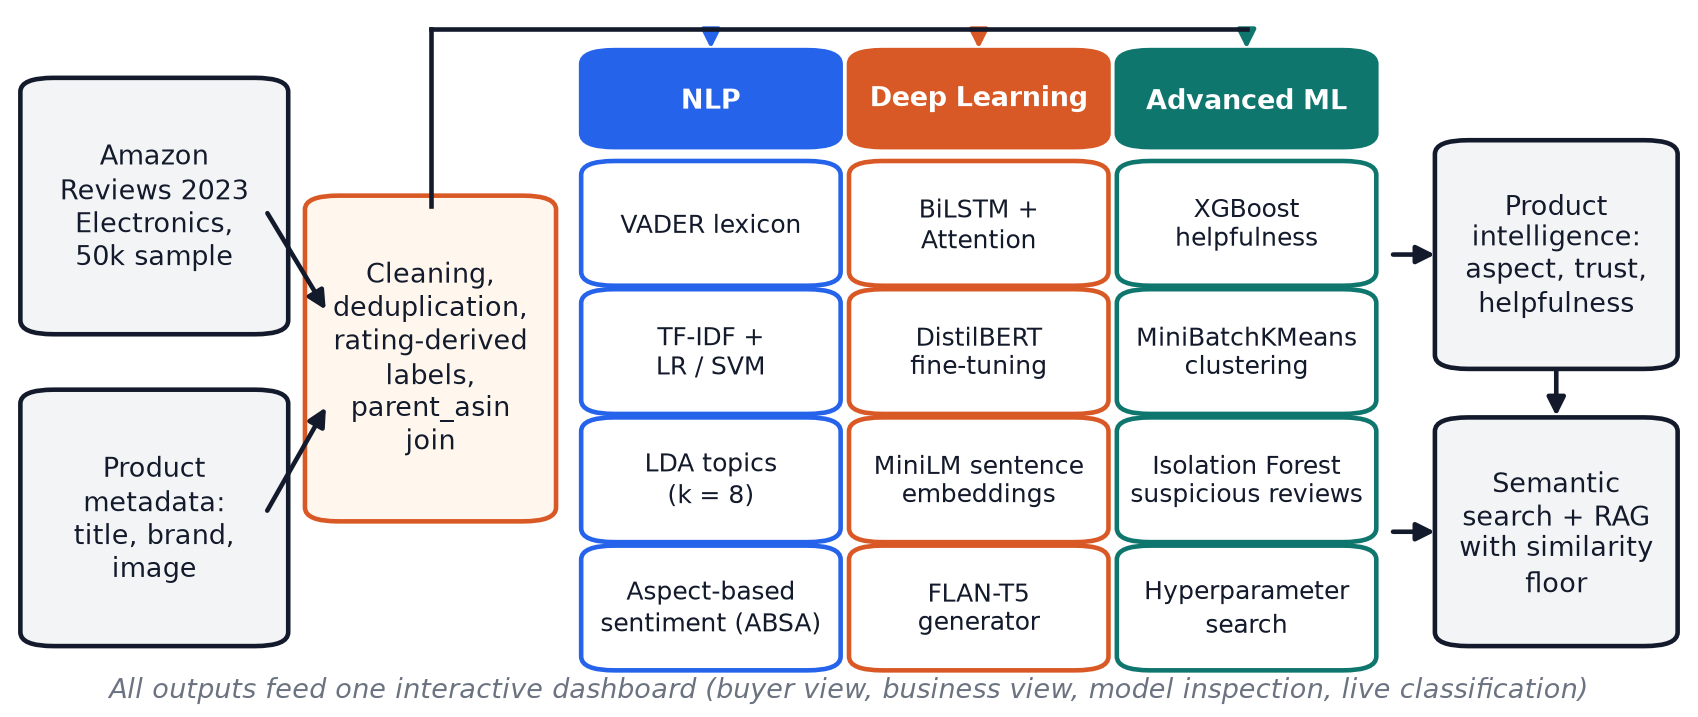
\includegraphics[width=0.86\textwidth]{figures/fig_framework.png}
\caption{The ReviewIQ framework. Reviews and product metadata are cleaned and joined, then processed by NLP, deep learning and advanced ML branches that feed product intelligence and a retrieval-augmented question-answering layer.}
\label{fig:framework}
\end{figure*}

\subsection{NLP branch}
\paragraph{Lexicon baseline} VADER \cite{hutto2014vader} produces a compound score $c\in[-1,1]$; we label $c\ge 0.05$ positive, $c\le -0.05$ negative and the rest neutral.
\paragraph{Feature-based classifiers} Reviews are vectorised with TF-IDF (unigrams and bigrams, 30{,}000 features, $\mathrm{min\_df}=2$, sublinear term frequency) and classified with multinomial logistic regression and a linear SVM, both with balanced class weights.
\paragraph{Topics} LDA \cite{blei2003lda} with $k=8$ topics is fit with online variational inference on a count matrix of 3{,}000 unigram and bigram features (stop words removed), using an 8{,}000-document subsample for fitting and applying the model to all reviews.
\paragraph{Aspect-based sentiment} Ten aspects (battery, camera, display, sound, performance, build quality, price/value, connectivity, size/comfort, customer service) are defined by keyword lexicons. Each review is split into sentences; sentences containing an aspect keyword are scored with VADER, and the aspect receives a positive, neutral or negative polarity. The matched sentences are retained as human-readable evidence for every aspect judgement.

\subsection{Deep learning branch}
\paragraph{BiLSTM with attention} Tokens (lower-cased alphanumerics plus ``!'' and ``?'') are mapped to a 14{,}937-word vocabulary built on the training split only (minimum frequency 3), and sequences are truncated to 200 tokens (Fig.~\ref{fig:lstm}). A learned 128-dimensional embedding feeds a two-layer bidirectional LSTM with 128 units per direction. With hidden states $\mathbf{h}_t$, attention pooling computes
\begin{equation}
\alpha_t=\frac{\exp(\mathbf{w}^{\top}\mathbf{h}_t)}{\sum_{s}\exp(\mathbf{w}^{\top}\mathbf{h}_s)},\qquad
\mathbf{c}=\sum_t \alpha_t \mathbf{h}_t,
\end{equation}
with padding positions masked, and $\mathbf{c}$ passes through dropout (0.4) and a linear layer to a three-way softmax. The model has 2.57\,M trainable parameters. Because the data are imbalanced, the cross-entropy loss uses class weights $w_c=\sqrt{N/(3n_c)}$, and the epoch is selected by validation macro-F1 rather than loss.

\begin{figure}[t]
\centering
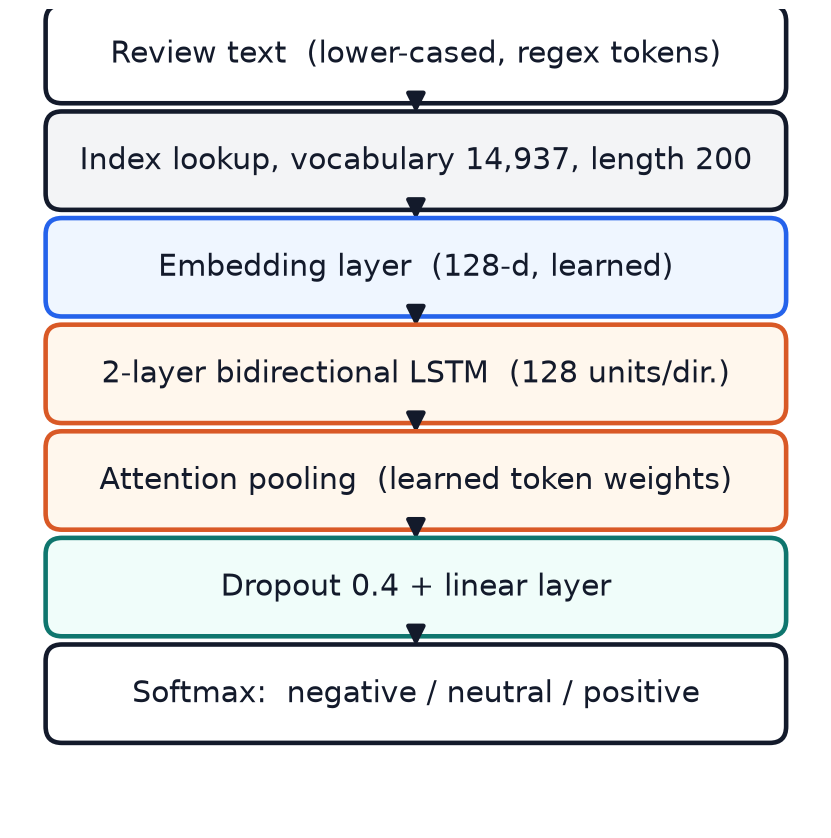
\includegraphics[width=0.78\columnwidth]{figures/fig_lstm_arch.png}
\caption{Architecture of the BiLSTM with attention pooling used for three-class sentiment classification.}
\label{fig:lstm}
\end{figure}

\paragraph{Fine-tuned DistilBERT} The pre-trained distilled transformer \cite{sanh2019distilbert} is fine-tuned with a three-way classification head (maximum length 128, the AdamW optimiser with learning rate $2\times10^{-5}$, 2 epochs, batch size 8) on a stratified 6{,}000-review subsample, because the run was performed on a CPU.

\subsection{Advanced ML branch}
\paragraph{Helpfulness prediction} The target is whether a review received at least one helpful vote. Ten engineered features are used: rating, length in words, title length, verified-purchase flag, exclamation and question-mark counts, capital-letter ratio, VADER compound score, review age in days, and the number of distinct aspects mentioned (taken from the ABSA output). An XGBoost classifier \cite{chen2016xgboost} is tuned with 15 randomised-search candidates under 3-fold cross-validation optimising F1, with \texttt{scale\_pos\_weight} set for the imbalance.
\paragraph{Clustering} MiniBatchKMeans with $k=6$ is run on a separate TF-IDF representation (5{,}000 features, stop words removed) so that function words do not dominate the clusters.
\paragraph{Suspicious-review detection} With no labelled fake/genuine data, we frame this as unsupervised anomaly detection. Features are: a binary indicator for very short reviews ($<10$ words), capital-letter ratio, exclamation count, verified-purchase flag, the logarithm of the number of reviews the same account has in the sample, and the maximum cosine similarity to another review of the same product (computed per product on sentence embeddings). After standardisation, an Isolation Forest \cite{liu2008isolation} with contamination 0.10 produces an anomaly score $s(x)=2^{-E[h(x)]/c(n)}$ that is rescaled to $[0,1]$. Rule-based reason strings accompany each flag for transparency. The interface describes flagged reviews only as \emph{potentially suspicious based on automated pattern analysis}.

\subsection{Semantic search and grounded question answering}
All reviews are encoded once with a MiniLM sentence encoder \cite{wang2020minilm,reimers2019sbert} into 384-dimensional unit vectors, so cosine similarity is a dot product. For a question $q$ about product $p$, retrieval is restricted to the reviews of $p$ (parent-ASIN scoping) and the top five by cosine similarity are returned. A FLAN-T5-base generator \cite{chung2022flan} is prompted with the question and the retrieved review text (each truncated to 300 characters) and asked to answer in one or two sentences using only that text. Because small generators do not reliably follow ``say you do not know'' instructions, we add a hard \emph{similarity floor}: if $\max_i\cos(q,r_i)<\tau$ with $\tau=0.30$, the system answers that the reviews do not provide enough information and does not call the generator. The retrieved reviews and their similarities are always displayed.

\subsection{Implementation}
The system is implemented in Python with PyTorch \cite{paszke2019pytorch}, scikit-learn \cite{pedregosa2011sklearn}, XGBoost, Transformers \cite{wolf2020transformers} and Streamlit. The dashboard offers buyer-oriented product pages (summaries, aspect evidence, filterable reviews, trust analysis, comparison, question answering), business views (complaint ranking, topics, review quality) and a live classifier that runs the LSTM, DistilBERT and SVM side by side with attention highlighting. Summaries and comparisons are generated from computed statistics by templates, never by a language model, so they cannot add unsupported claims.

\section{Experimental Setup}
\subsection{Protocol}
All sentiment models are evaluated on one stratified 80/20 split (random seed 42), giving 40{,}000 training and 10{,}000 test reviews. For the LSTM, 10\% of the training portion (4{,}000 reviews) is held out for early stopping, leaving 36{,}000 for gradient updates; the test set is never used for model selection. VADER needs no training and is scored on the same 10{,}000 test reviews. We report accuracy and macro-F1 with 95\% percentile bootstrap confidence intervals (2{,}000 resamples of the test set) \cite{efron1993bootstrap}, and paired bootstrap differences between models computed on the same resamples.

\subsection{Training details}
The LSTM is trained with Adam \cite{kingma2015adam} (learning rate $2\times10^{-3}$, weight decay $10^{-5}$), batch size 128, gradient clipping at 1.0, for at most 12 epochs with early stopping (patience 3). Training took about seven minutes on an NVIDIA RTX 4050 laptop GPU. DistilBERT was fine-tuned on CPU in about 60 minutes. Software versions for the LSTM and evaluation runs were PyTorch 2.13, scikit-learn 1.9, XGBoost 3.4 and Transformers 5.16 on Python 3.12; the DistilBERT fine-tuning run used the same code on an earlier installation.

\subsection{Ablation protocol}
To separate the contribution of the architecture from that of the loss weighting, we trained three LSTM variants with three random seeds each (42, 43, 44): the full model; the same model with an unweighted cross-entropy loss; and a variant that replaces attention pooling with masked mean pooling over the LSTM outputs (weighted loss retained). Only the seed changes between runs; the data split, vocabulary and test set are identical to the main experiment. We report mean and standard deviation over seeds.

\subsection{Metrics}
For class $c$ with precision $P_c$ and recall $R_c$, $F1_c=2P_cR_c/(P_c+R_c)$ and macro-F1 is $\frac{1}{3}\sum_c F1_c$, which weights the 7\% neutral class equally with the 80\% positive class.

\subsection{Reproducibility}
All reported numbers are regenerated from saved artefacts by scripts (data preparation, per-model training, the ablation runner and a shared evaluation script) with fixed seeds: 42 for the splits and the reported LSTM, and 42, 43 and 44 for the ablation.

\section{Results and Discussion}
\subsection{Sentiment classification}
Table~\ref{tab:main} and Fig.~\ref{fig:ci} give the main comparison. Every trained model clearly outperforms the lexicon baseline, whose neutral-class F1 is only 0.08: VADER assigns the neutral label to few reviews, whereas ``neutral'' in rating space often means mixed or lukewarm text.

\begin{table}[t]
\caption{Sentiment results on the shared 10{,}000-review test set. Accuracy and macro-F1 are given with the half-width of the 95\% bootstrap CI; best value per column in bold.}
\label{tab:main}
\centering
\footnotesize
\setlength{\tabcolsep}{3pt}
\begin{tabular}{@{}lccccc@{}}
\toprule
Model & Accuracy & Macro-F1 & F1$_{neg}$ & F1$_{neu}$ & F1$_{pos}$ \\
\midrule
VADER & .813$\pm$.008 & .512$\pm$.012 & .551 & .080 & .906 \\
TF-IDF + LR & .860$\pm$.007 & .689$\pm$.013 & .733 & .400 & .935 \\
TF-IDF + SVM & .888$\pm$.006 & .693$\pm$.014 & .747 & .382 & .950 \\
BiLSTM + Attn. & .888$\pm$.006 & \textbf{.718}$\pm$.013 & .754 & \textbf{.446} & .954 \\
DistilBERT & \textbf{.899}$\pm$.006 & .702$\pm$.015 & \textbf{.780} & .368 & \textbf{.958} \\
\bottomrule
\end{tabular}
\end{table}

\begin{figure}[t]
\centering
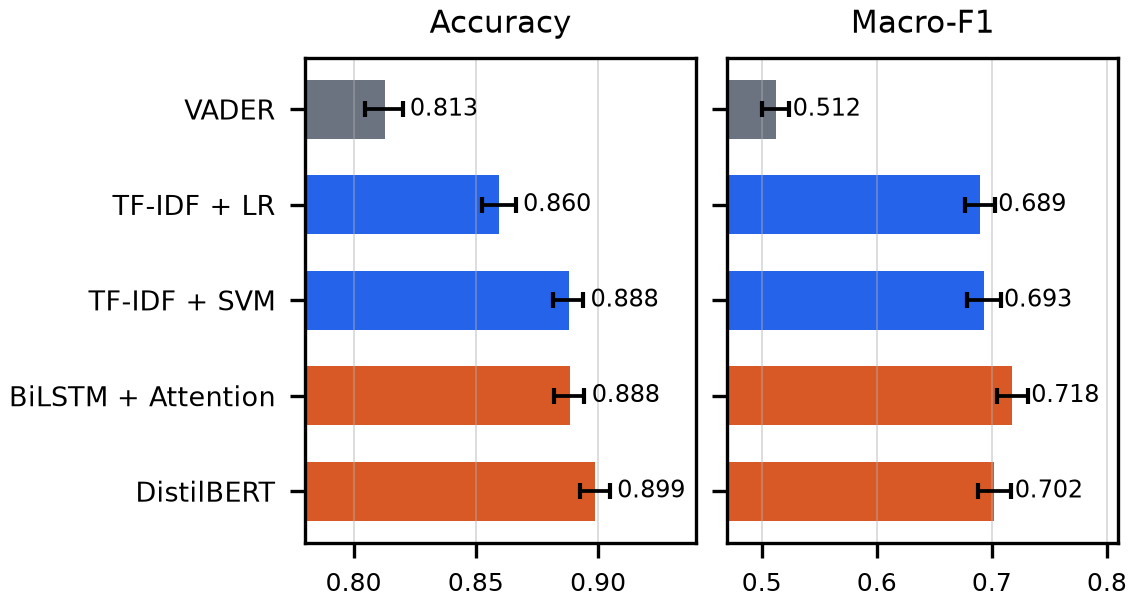
\includegraphics[width=\columnwidth]{figures/fig_model_ci.png}
\caption{Accuracy and macro-F1 with 95\% bootstrap confidence intervals on the shared test set. Deep models are shown in orange.}
\label{fig:ci}
\end{figure}

The two neural models are the strongest, but in different ways. DistilBERT has the highest accuracy and negative/positive F1, while the BiLSTM has the highest macro-F1 because it recovers the neutral class better (F1 0.446 versus 0.368 for DistilBERT and 0.382 for the SVM). Paired bootstrap tests (Table~\ref{tab:paired}) qualify these statements: the BiLSTM's macro-F1 advantage over the SVM is significant, its advantage over DistilBERT is borderline and not significant at the 95\% level, and DistilBERT's accuracy advantage over both is significant. Notably, the BiLSTM and the SVM are indistinguishable in accuracy; the neural model's gain is concentrated on minority classes.

\begin{table}[t]
\caption{Paired bootstrap differences (first model minus second) with 95\% intervals, 2{,}000 resamples. Intervals excluding zero are significant.}
\label{tab:paired}
\centering
\footnotesize
\setlength{\tabcolsep}{1.5pt}
\begin{tabular}{@{}lcc@{}}
\toprule
Comparison & $\Delta$ Macro-F1 [CI] & $\Delta$ Accuracy [CI] \\
\midrule
BiLSTM $-$ SVM & +.025 [+.010,+.039] & +.001 [$-$.005,+.006] \\
BiLSTM $-$ DistilBERT & +.016 [$-$.000,+.031] & $-$.011 [$-$.016,$-$.005] \\
DistilBERT $-$ SVM & +.009 [$-$.008,+.026] & +.011 [+.005,+.017] \\
\bottomrule
\end{tabular}
\end{table}

Two caveats prevent over-interpretation. First, the TF-IDF models and the LSTM all use class weighting, which is known to raise macro-F1 at some cost to accuracy, whereas DistilBERT was trained without it; the ablation in Section~VI-C quantifies this effect for the LSTM. Second, DistilBERT saw 6{,}000 training reviews against 36{,}000 for the LSTM, so its numbers are best read as a lower bound on what a fully fine-tuned transformer would achieve. The ranking should therefore be taken as a statement about these specific training budgets and loss functions, not about the architectures in general.

Fig.~\ref{fig:cm} shows the BiLSTM's training dynamics and confusion matrix. Training loss falls monotonically while validation macro-F1 plateaus after epoch three and peaks at epoch six, after which the validation metrics stop improving while training loss keeps falling and early stopping triggers. Most errors involve the neutral class: 191 of the 701 neutral reviews are predicted positive and 148 negative, while 331 of the 8{,}041 positive reviews are predicted neutral, reflecting how ambiguous text is pulled towards the dominant positive class.

\begin{figure*}[t]
\centering
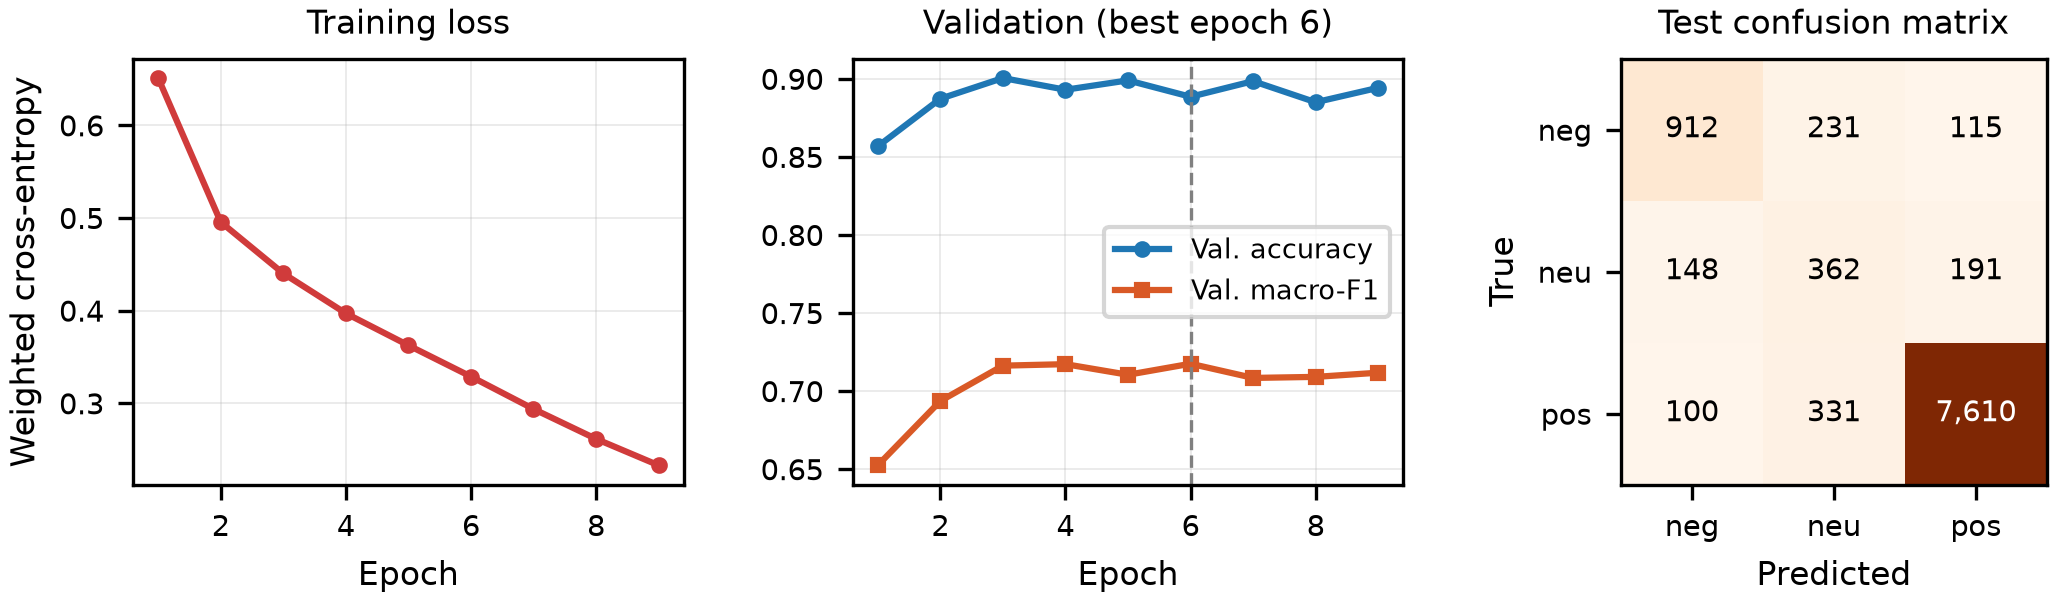
\includegraphics[width=0.84\textwidth]{figures/fig_dl_results.png}
\caption{BiLSTM training dynamics (left, middle) and test-set confusion matrix (right). Validation macro-F1 peaks at epoch six, after which early stopping ends training.}
\label{fig:cm}
\end{figure*}

\subsection{Error analysis}
The reported BiLSTM makes 1{,}116 errors on the 10{,}000 test reviews (11.2\%), of which 155 are confident (predicted probability of at least 0.90). Of these, 98 involve the neutral class (75 neutral reviews read as positive, 23 as negative), 48 are polar opposites (36 negative reviews predicted positive and 12 positive reviews predicted negative), and 9 are other mixes. Table~\ref{tab:errors} shows illustrative cases that we selected from the confident polar-opposite errors; we did not audit them systematically. In these cases the star rating contradicts the text, so a part of the apparent error is label noise rather than model failure, and the measured accuracy and macro-F1 understate how well the model tracks what reviewers actually wrote.

\begin{table}[t]
\caption{Confident disagreements between star rating and the BiLSTM (probability in brackets). Excerpts are verbatim.}
\label{tab:errors}
\centering
\footnotesize
\begin{tabularx}{\columnwidth}{@{}>{\raggedright\arraybackslash}p{2.15cm}X@{}}
\toprule
Stars / predicted & Review excerpt \\
\midrule
5 / negative (.99) & ``Piece of junk !!! Poor quality, high price .. it lasted 10weeks'' \\
5 / negative (.98) & ``Poor quality ties. Dont waste your money. Small and wont latch at all'' \\
2 / positive (1.00) & ``This was an excellent remote. Excellent remote'' \\
1 / positive (1.00) & ``Worked out of the box. love it'' \\
\bottomrule
\end{tabularx}
\end{table}

\subsection{Ablation: what drives the BiLSTM's gain?}
Two design choices could explain the BiLSTM's macro-F1 advantage: attention pooling and the class-weighted loss. Table~\ref{tab:ablation} reports the three variants over three seeds.

\begin{table}[t]
\caption{LSTM ablation on the shared test set (mean $\pm$ std over three seeds). The DistilBERT row is a single run for reference.}
\label{tab:ablation}
\centering
\footnotesize
\setlength{\tabcolsep}{3pt}
\begin{tabular}{@{}lccc@{}}
\toprule
Variant & Accuracy & Macro-F1 & F1$_{neu}$ \\
\midrule
Full (attention + class weights) & .891$\pm$.003 & \textbf{.722}$\pm$.004 & \textbf{.445}$\pm$.000 \\
No class weights & \textbf{.899}$\pm$.001 & .709$\pm$.008 & .405$\pm$.013 \\
Mean pooling (class weights) & .889$\pm$.003 & .715$\pm$.005 & .430$\pm$.004 \\
\midrule
DistilBERT (reference) & .899 & .702 & .368 \\
\bottomrule
\end{tabular}
\end{table}

Class weighting is the dominant factor. Removing it lowers macro-F1 by 0.012 on average (by 0.003, 0.011 and 0.023 across the three seeds) and lowers neutral-class F1 from 0.445 to 0.405, but raises accuracy by 0.007 on average, with the same sign in every seed. Replacing attention with mean pooling lowers macro-F1 by 0.007 on average (0.001 to 0.015 across seeds) and leaves accuracy unchanged within noise. Attention therefore contributes a small and less consistent improvement; with three seeds per variant we do not test its significance and report only the sign consistency.

Two consequences follow. First, the seed-to-seed standard deviation of the full model (about 0.004 macro-F1) is much smaller than its gap to the TF-IDF SVM (about 0.03), so that advantage is not a seed artefact. Second, an LSTM trained without class weights matches DistilBERT's accuracy (0.899 versus 0.899) while still exceeding its macro-F1 on average (0.709 versus 0.702). This suggests that DistilBERT's apparent accuracy lead in Table~\ref{tab:main} owes more to the choice of operating point on the accuracy/macro-F1 trade-off than to a clear difference in capacity, although DistilBERT was trained only once and on a sixth of the data.

\subsection{Computational cost}
Accuracy is only one axis for a deployed system. Table~\ref{tab:cost} gives parameter counts and measured throughput for the three trained sentiment models on test-split reviews, including tokenisation or vectorisation, after a warm-up run and taking the best of repeated runs. The GPU is the laptop RTX 4050 used for training; CPU figures use the same machine (8 logical cores). DistilBERT was timed on 200 reviews on CPU and 1{,}000 on GPU.

\begin{table}[t]
\caption{Model size and inference throughput (reviews per second).}
\label{tab:cost}
\centering
\footnotesize
\begin{tabular}{@{}lccc@{}}
\toprule
Model & Parameters & CPU & GPU \\
\midrule
TF-IDF + SVM & 90\,k & 13{,}550 & n/a \\
BiLSTM + Attention & 2.57\,M & 975 & 5{,}688 \\
DistilBERT & 66.96\,M & 17 & 451 \\
\bottomrule
\end{tabular}
\end{table}

The BiLSTM has 26 times fewer parameters than DistilBERT and classifies about 57 times faster on CPU (975 versus 17 reviews per second) and 13 times faster on GPU. It trails DistilBERT by about one accuracy point in its class-weighted form and matches it when trained without class weights (Section~VI-C), so for batch-scoring large review catalogues or serving on CPU-only hardware it offers a much better balance of cost and accuracy, whereas the SVM is fastest but has the lowest macro-F1 of the three. A transformer fine-tuned on more data would likely narrow the accuracy gap, but not the cost gap.

\subsection{Language of each sentiment}
Word clouds (Fig.~\ref{fig:wc}) weight each word by its within-class frequency multiplied by its over-representation relative to the whole corpus, so they show distinctive rather than merely frequent vocabulary. Negative reviews are dominated by return and failure language (``return'', ``waste'', ``money'', ``stopped'', ``broke''), positive reviews by ease and satisfaction (``easy'', ``love'', ``nice'', ``perfect''), and neutral reviews by hedged evaluation (``okay'', ``fine'', ``better'', ``bit'') mixed with product nouns, which is consistent with the difficulty of the neutral class.

\begin{figure*}[t]
\centering
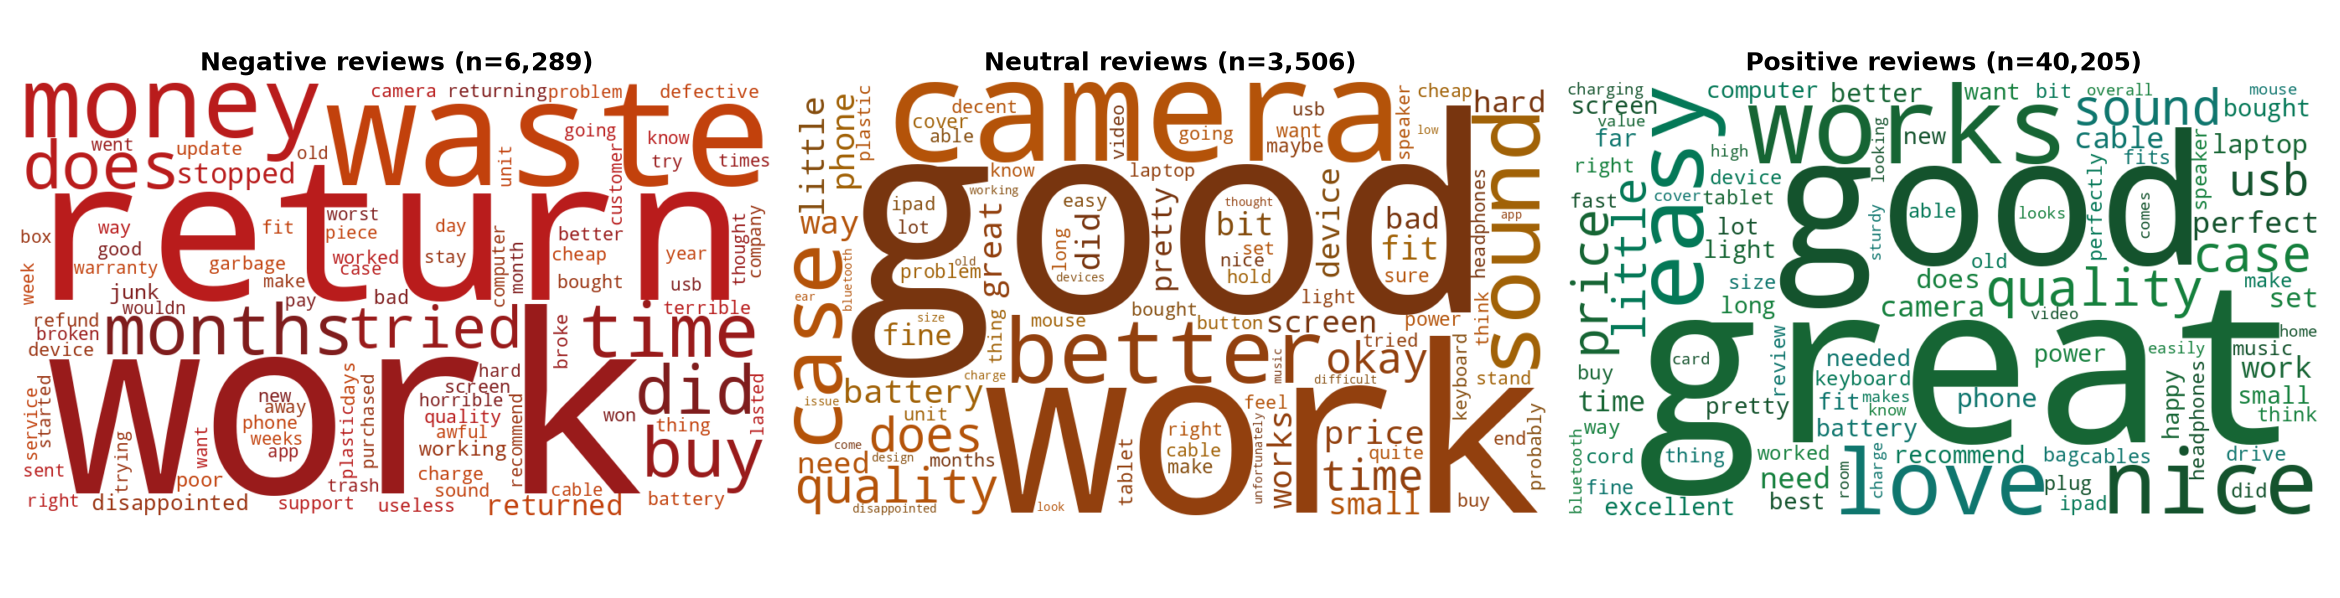
\includegraphics[width=0.80\textwidth]{figures/wordcloud_all_sentiments.png}
\caption{Distinctive-vocabulary word clouds for negative, neutral and positive reviews.}
\label{fig:wc}
\end{figure*}

\subsection{Aspect-level intelligence}
The lexicon matched 64{,}134 aspect mentions in 33{,}257 reviews (66.5\%). Table~\ref{tab:aspect} ranks aspects by negative share. Battery is the most criticised aspect at 20.2\% negative mentions, followed by connectivity (19.3\%) and customer service (19.3\%), while build quality draws the lowest negative share (8.1\%). Because the aspect sentiment is computed on matched sentences rather than whole reviews, a single review can be positive about sound and negative about battery, which a single review-level label cannot express. In the live classifier a sentence such as ``the battery is terrible but the sound quality is amazing'' receives three different review-level labels from the three classifiers, illustrating why aspect-level analysis is complementary to, not redundant with, sentiment classification.

\begin{table}[t]
\caption{Aspect-level sentiment (\% of mentions), ranked by negative share.}
\label{tab:aspect}
\centering
\footnotesize
\begin{tabular}{@{}lrrrr@{}}
\toprule
Aspect & Pos. & Neu. & Neg. & Mentions \\
\midrule
Battery & 56.3 & 23.5 & 20.2 & 6{,}968 \\
Connectivity & 56.7 & 23.9 & 19.3 & 4{,}166 \\
Customer service & 64.0 & 16.7 & 19.3 & 2{,}958 \\
Performance & 58.7 & 25.5 & 15.8 & 4{,}726 \\
Display & 64.4 & 21.1 & 14.5 & 4{,}540 \\
Sound & 73.4 & 13.7 & 12.9 & 8{,}327 \\
Camera & 70.1 & 18.6 & 11.3 & 5{,}991 \\
Price/value & 74.2 & 15.1 & 10.7 & 11{,}070 \\
Size/comfort & 76.1 & 13.5 & 10.4 & 10{,}752 \\
Build quality & 66.5 & 25.4 & 8.1 & 4{,}636 \\
\bottomrule
\end{tabular}
\end{table}

\subsection{Topics and clusters}
The eight LDA topics separate along product families: audio and speakers; storage cards and Apple accessories; general praise with computers and drives; USB and power accessories; cameras, televisions and mounts; cases and tablets; headphones and phones; and cables and networking. Clustering is less informative. Of six KMeans clusters, only two are clearly topical (laptop bags and cases, 5{,}101 reviews; sound and headphones, 5{,}240 reviews); the remaining four are dominated by generic praise (``works great'', ``five stars'', ``great product'') and have mean ratings between 4.0 and 4.8. We report this as a negative finding: on short, rating-skewed reviews, TF-IDF clustering mostly recovers sentiment style rather than subject, and LDA is the better tool for discovering topics.

\subsection{Helpfulness prediction}
The tuned XGBoost model (best configuration: 200 trees, depth 6, learning rate 0.01, subsample 0.7, column sample 0.7) reaches 70.5\% accuracy on the test set with helpful-class precision 0.458, recall 0.702 and F1 0.555. Accuracy is modest in absolute terms; helpfulness is a noisy target that plausibly depends on exposure (how many people saw the review), which no review-level feature captures. Feature importance (Fig.~\ref{fig:aspects}b) is led by review length, followed by the number of distinct aspects mentioned and the rating, suggesting that longer, more informative reviews attract more votes; the aspect-count feature, produced by the ABSA module, ranks second, showing how one component feeds another.

\begin{figure*}[t]
\centering
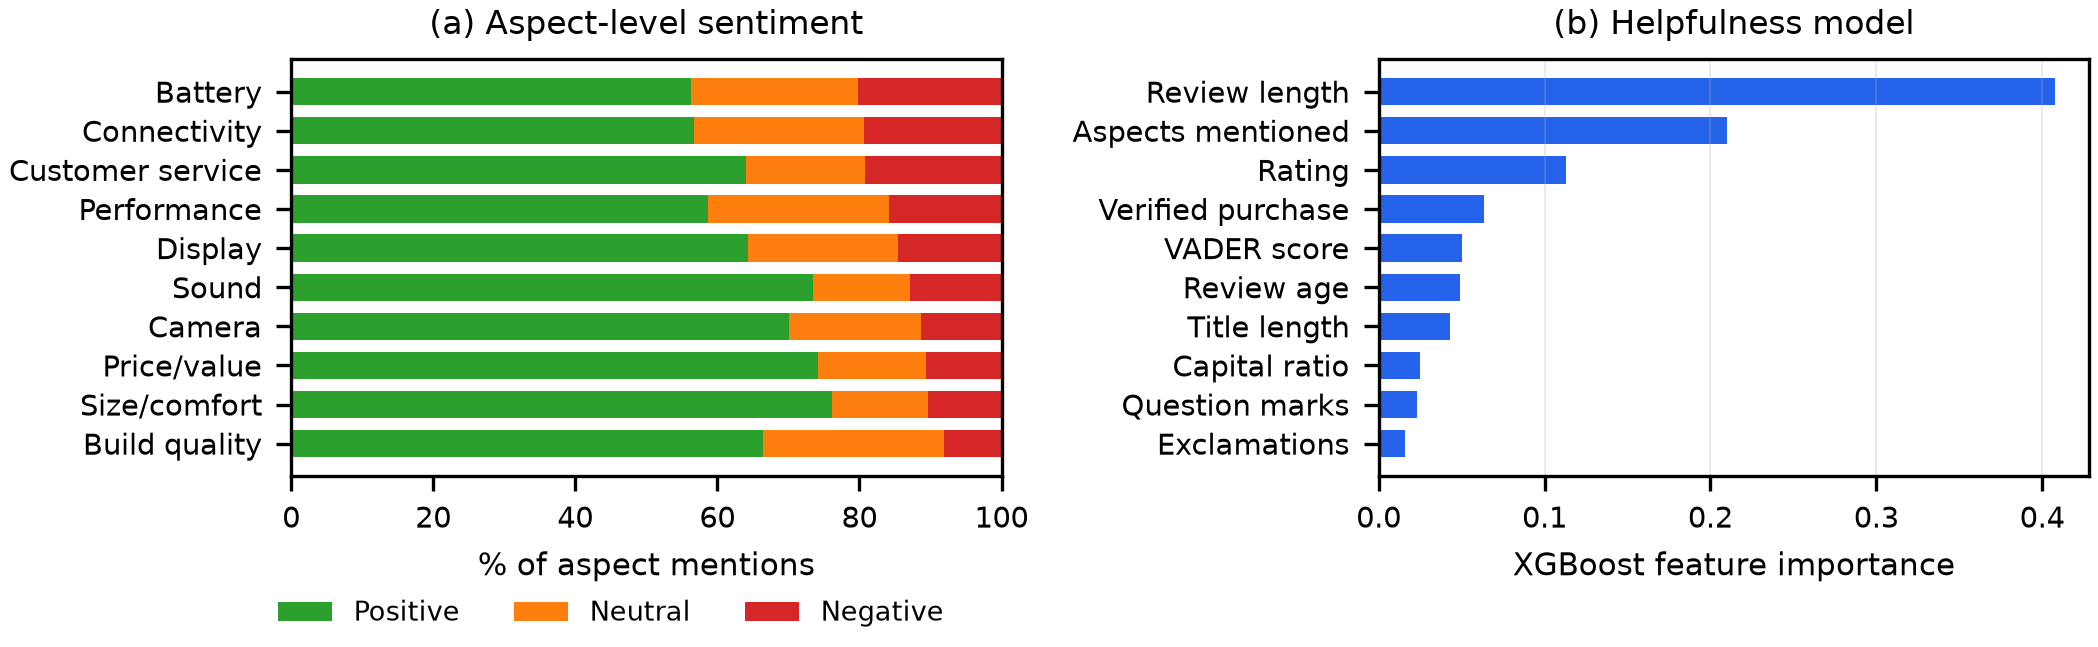
\includegraphics[width=0.84\textwidth]{figures/fig_aspects_importance.png}
\caption{(a) Aspect-level sentiment shares, sorted by negative share. (b) XGBoost feature importance for helpfulness prediction.}
\label{fig:aspects}
\end{figure*}

\subsection{Suspicious-review detection}
With no ground truth we cannot report accuracy, and we do not. The Isolation Forest flags 4{,}999 reviews (10.0\%), of which 36 are near-duplicates (cosine similarity $\ge0.95$ within a product). Inspection of the flagged set is nevertheless instructive. An earlier feature set that fed raw rating and raw length into the forest produced scores correlated $+0.55$ with length and $-0.42$ with rating: the model was flagging long, detailed, negative reviews, which are rare but not suspicious. Replacing raw length with a ``very short'' indicator, removing rating, and adding the per-account review count reversed this; the new scores correlate $+0.06$ with length and $+0.25$ with account volume. The highest-scoring reviews are now templated one-liners (``Five Stars. Love it!!!''), all-capitals emotional text, and effusive praise from high-volume unverified accounts. The lesson is general: isolation-based methods flag statistical rarity, so features must be chosen so that rarity aligns with the behaviour of interest.

\subsection{Retrieval and the similarity floor}
\paragraph{Retrieval} We wrote one paraphrased query per aspect that deliberately avoids every keyword in the aspect lexicon (e.g., ``I have to plug it in twice a day or it just dies'') and counted how many of the top five reviews mention the aspect. Dense retrieval achieved a mean aspect-mention rate of 0.54 against 0.32 for TF-IDF retrieval (Table~\ref{tab:retr}). The advantage is not uniform: dense retrieval was better on seven aspects (camera, sound, performance, build quality, price/value, connectivity, size/comfort), tied on customer service, worse on display, and both methods scored zero on the battery query. With ten queries the difference is indicative, not conclusive, and the lexicon-based relevance proxy under-counts relevant reviews that use other wording, so both rates are lower bounds.

\begin{table}[t]
\caption{Retrieval and guardrail results.}
\label{tab:retr}
\centering
\footnotesize
\begin{tabular}{@{}lcc@{}}
\toprule
\multicolumn{3}{@{}l}{\textit{(a) Aspect-mention rate@5 (10 paraphrased queries)}}\\
Method & Mean & Queries $\ge0.6$ \\
\midrule
TF-IDF cosine & 0.32 & 3 / 10 \\
MiniLM dense & 0.54 & 6 / 10 \\
\midrule
\multicolumn{3}{@{}l}{\textit{(b) Top-1 similarity (9 products $\times$ 5 questions)}}\\
Question group & Mean & Below $\tau$ \\
\midrule
Answerable & 0.455 & 2.2\% \\
Plausible but unanswerable & 0.218 & 95.6\% \\
Off-topic & 0.184 & 100\% \\
\bottomrule
\end{tabular}
\end{table}

\paragraph{Guardrail} Table~\ref{tab:retr}(b) shows that top-1 similarity separates answerable from unanswerable questions well: with $\tau=0.30$ the system declines 100\% of off-topic and 95.6\% of plausible-but-unanswerable questions (for example warranty, colour options or waterproof ratings the reviews never mention) while declining only 2.2\% of answerable ones. The guardrail was introduced after we observed the unguarded generator answering ``No'' to a warranty question at a top-1 similarity of about 0.25, i.e.\ producing a confident but ungrounded answer. We evaluated the guardrail on 45 product and question pairs per group across the nine products with at least 60 reviews, so the estimate has wide uncertainty; and we did not evaluate the faithfulness of answers that pass the floor, which remains future work.

\subsection{Practical implications}
The results suggest how each audience can use the system. A buyer gains most from the aspect view, which replaces a single star average with evidence-linked statements, and from question answering that can say the reviews are silent. A seller gains from the complaint ranking (battery, connectivity, customer service) and the review-quality view.

\section{Limitations and Threats to Validity}
\paragraph{Weak labels} Sentiment is derived from stars, not human annotation; reported accuracies measure agreement with ratings. Manual annotation of a subset would give a cleaner neutral class.
\paragraph{Sampling} The working sample was taken from the beginning of the category file rather than drawn at random. That file is grouped by reviewer (the 65{,}552 raw records form 9{,}686 contiguous blocks, one per reviewer), so the sample over-represents prolific reviewers: 392 accounts with at least 20 reviews contribute about 40\% of it. This distorts per-account features such as the one used for suspicious-review detection, and it limits generalisation to the full catalogue. Results are for English-language reviews in a single product category and may not transfer to other languages or domains.
\paragraph{Unequal training budgets} DistilBERT was fine-tuned on one-sixth of the data used for the LSTM and without class weighting. The main comparison uses a single training run per model; the bootstrap intervals capture test-sampling variance, and the ablation shows that the LSTM's seed-to-seed standard deviation is small (about 0.004 macro-F1 and 0.003 accuracy), but DistilBERT was trained only once.
\paragraph{Lexicon-based aspects} The ABSA module relies on keyword lexicons and sentence-level VADER scores, so it misses implicit aspects and can mis-score sarcasm or negation. Aspect polarity was not validated against human labels.
\paragraph{No ground truth for suspicion} Flagged reviews are anomalies, not confirmed fakes, and the interface is worded accordingly. Coordinated campaigns that imitate normal behaviour would not be detected.
\paragraph{Evaluation of generation} We measured retrieval and the refusal guardrail but not the faithfulness or fluency of generated answers.

\section{Conclusion}
We presented ReviewIQ, a framework that integrates NLP, deep learning and advanced machine learning around a shared review corpus and exposes the results through a grounded, product-scoped dashboard. A BiLSTM with attention trained from scratch matched a TF-IDF SVM in accuracy but significantly improved macro-F1 by better recognising the neutral class, while a lightly fine-tuned DistilBERT gave the best accuracy of the default-trained models; the two neural models were statistically comparable on macro-F1. A three-seed ablation showed that class weighting, rather than attention pooling, accounts for most of the LSTM's macro-F1 gain at a small cost in accuracy, and that an unweighted LSTM matches DistilBERT's accuracy. The LSTM also runs about 57 times faster than DistilBERT on CPU with 26 times fewer parameters. Aspect analysis identified battery, connectivity and customer service as the main complaint areas, helpfulness could be predicted moderately well from review structure, and an unsupervised anomaly score surfaced low-effort and high-volume review patterns once its features were corrected. A similarity floor made the question-answering component decline nearly all unsupported questions. Future work includes training DistilBERT on the full data with matched class weighting, learned aspect extraction, human-annotated neutral and suspicious subsets, random rather than contiguous sampling across categories, a faithfulness evaluation of generated answers, larger generators for the question-answering component, and a seller-facing view that tracks complaint areas over time.

\section*{Acknowledgment}
The authors thank Prof. Sneha Annappanavar for her guidance, and the maintainers of the Amazon Reviews 2023 collection.

\balance
\begin{thebibliography}{99}
\bibitem{pang2002thumbs} B. Pang, L. Lee, and S. Vaithyanathan, ``Thumbs up? Sentiment classification using machine learning techniques,'' in \emph{Proc. EMNLP}, 2002, pp. 79--86.
\bibitem{liu2012sentiment} B. Liu, \emph{Sentiment Analysis and Opinion Mining}. San Rafael, CA, USA: Morgan \& Claypool, 2012.
\bibitem{hu2004mining} M. Hu and B. Liu, ``Mining and summarizing customer reviews,'' in \emph{Proc. ACM SIGKDD}, 2004, pp. 168--177.
\bibitem{kim2006automatically} S.-M. Kim, P. Pantel, T. Chklovski, and M. Pennacchiotti, ``Automatically assessing review helpfulness,'' in \emph{Proc. EMNLP}, 2006, pp. 423--430.
\bibitem{jindal2008opinion} N. Jindal and B. Liu, ``Opinion spam and analysis,'' in \emph{Proc. WSDM}, 2008, pp. 219--230.
\bibitem{ott2011finding} M. Ott, Y. Choi, C. Cardie, and J. T. Hancock, ``Finding deceptive opinion spam by any stretch of the imagination,'' in \emph{Proc. ACL}, 2011, pp. 309--319.
\bibitem{joachims1998text} T. Joachims, ``Text categorization with support vector machines: Learning with many relevant features,'' in \emph{Proc. ECML}, 1998, pp. 137--142.
\bibitem{hutto2014vader} C. J. Hutto and E. Gilbert, ``VADER: A parsimonious rule-based model for sentiment analysis of social media text,'' in \emph{Proc. ICWSM}, 2014.
\bibitem{hochreiter1997lstm} S. Hochreiter and J. Schmidhuber, ``Long short-term memory,'' \emph{Neural Computation}, vol. 9, no. 8, pp. 1735--1780, 1997.
\bibitem{bahdanau2015attention} D. Bahdanau, K. Cho, and Y. Bengio, ``Neural machine translation by jointly learning to align and translate,'' in \emph{Proc. ICLR}, 2015.
\bibitem{wang2016attention} Y. Wang, M. Huang, X. Zhu, and L. Zhao, ``Attention-based LSTM for aspect-level sentiment classification,'' in \emph{Proc. EMNLP}, 2016, pp. 606--615.
\bibitem{devlin2019bert} J. Devlin, M.-W. Chang, K. Lee, and K. Toutanova, ``BERT: Pre-training of deep bidirectional transformers for language understanding,'' in \emph{Proc. NAACL-HLT}, 2019, pp. 4171--4186.
\bibitem{sanh2019distilbert} V. Sanh, L. Debut, J. Chaumond, and T. Wolf, ``DistilBERT, a distilled version of BERT: smaller, faster, cheaper and lighter,'' arXiv:1910.01108, 2019.
\bibitem{blei2003lda} D. M. Blei, A. Y. Ng, and M. I. Jordan, ``Latent Dirichlet allocation,'' \emph{J. Mach. Learn. Res.}, vol. 3, pp. 993--1022, 2003.
\bibitem{chen2016xgboost} T. Chen and C. Guestrin, ``XGBoost: A scalable tree boosting system,'' in \emph{Proc. ACM SIGKDD}, 2016, pp. 785--794.
\bibitem{liu2008isolation} F. T. Liu, K. M. Ting, and Z.-H. Zhou, ``Isolation forest,'' in \emph{Proc. IEEE ICDM}, 2008, pp. 413--422.
\bibitem{reimers2019sbert} N. Reimers and I. Gurevych, ``Sentence-BERT: Sentence embeddings using Siamese BERT-networks,'' in \emph{Proc. EMNLP-IJCNLP}, 2019, pp. 3982--3992.
\bibitem{wang2020minilm} W. Wang, F. Wei, L. Dong, H. Bao, N. Yang, and M. Zhou, ``MiniLM: Deep self-attention distillation for task-agnostic compression of pre-trained transformers,'' in \emph{Proc. NeurIPS}, vol. 33, 2020, pp. 5776--5788.
\bibitem{lewis2020rag} P. Lewis \emph{et al.}, ``Retrieval-augmented generation for knowledge-intensive NLP tasks,'' in \emph{Proc. NeurIPS}, vol. 33, 2020, pp. 9459--9474.
\bibitem{raffel2020t5} C. Raffel \emph{et al.}, ``Exploring the limits of transfer learning with a unified text-to-text transformer,'' \emph{J. Mach. Learn. Res.}, vol. 21, no. 140, pp. 1--67, 2020.
\bibitem{chung2022flan} H. W. Chung \emph{et al.}, ``Scaling instruction-finetuned language models,'' arXiv:2210.11416, 2022.
\bibitem{hou2024bridging} Y. Hou \emph{et al.}, ``Bridging language and items for retrieval and recommendation,'' arXiv:2403.03952, 2024.
\bibitem{kingma2015adam} D. P. Kingma and J. Ba, ``Adam: A method for stochastic optimization,'' in \emph{Proc. ICLR}, 2015.
\bibitem{paszke2019pytorch} A. Paszke \emph{et al.}, ``PyTorch: An imperative style, high-performance deep learning library,'' in \emph{Proc. NeurIPS}, vol. 32, 2019, pp. 8024--8035.
\bibitem{pedregosa2011sklearn} F. Pedregosa \emph{et al.}, ``Scikit-learn: Machine learning in Python,'' \emph{J. Mach. Learn. Res.}, vol. 12, pp. 2825--2830, 2011.
\bibitem{wolf2020transformers} T. Wolf \emph{et al.}, ``Transformers: State-of-the-art natural language processing,'' in \emph{Proc. EMNLP: System Demonstrations}, 2020, pp. 38--45.
\bibitem{efron1993bootstrap} B. Efron and R. J. Tibshirani, \emph{An Introduction to the Bootstrap}. New York, NY, USA: Chapman \& Hall, 1993.
\end{thebibliography}

\end{document}
